\documentclass[11pt]{article}
% Build: latexmk -pdf main.tex   (or: tectonic main.tex)
% Figures are already rendered to PDF. figures/make_figures.py redraws them from figures/data/.

\usepackage[T1]{fontenc}
\usepackage[utf8]{inputenc}
\usepackage{lmodern}
\usepackage[margin=1in]{geometry}
\usepackage{microtype}
\usepackage{graphicx}
\usepackage{booktabs}
\usepackage{tabularx}
\usepackage{array}
\usepackage{xcolor}
\usepackage{listings}
\usepackage{enumitem}
\usepackage[numbers,sort&compress]{natbib}
\usepackage{caption}
\usepackage[colorlinks=true,linkcolor=blue!50!black,citecolor=blue!50!black,urlcolor=blue!50!black]{hyperref}

\graphicspath{{figures/}}
\captionsetup{font=small,labelfont=bf}
\newcolumntype{Y}{>{\raggedright\arraybackslash}X}
\newcommand{\code}[1]{\texttt{\detokenize{#1}}}

\lstset{basicstyle=\ttfamily\footnotesize,breaklines=true,columns=fullflexible,
  frame=single,framerule=0.4pt,rulecolor=\color{black!35},xleftmargin=4pt,xrightmargin=4pt,
  breakindent=0pt}

\title{Is Hindsight Really 20/20?}
\author{Benjamin Ebanks}
\date{November 5, 2026}

\begin{document}
\maketitle

\section{Introduction}
\label{sec:intro}

Tools such as Claude Code, Codex and OpenCode give a language model an environment in which it can work as an engineer's daily assistant, taking requests and completing them as they come. These agents struggle as requirements accumulate. On EvoCode-Bench, pass rates fall below half of round-1 performance by round 5~\cite{shen2026evocode}. On SlopCodeBench, structural erosion rises in 77\% of trajectories~\cite{orlanski2026slopcode}. The problem appears to sit in the code as well as the conversation: ChainSWE finds that inherited repository state accounts for most of the decline~\cite{jin2026chainswe}, and SlopCodeBench reports that quality prompts lower the starting point of degradation but not its rate. Both suggest that revisiting the design is a research direction worth exploring.

Any engineer knows the feeling behind those numbers. By the tenth request you can see how you would have designed your system if you had known all of the requirements, but you are too far in, and you have a next request to get to. You could copy all of your requirements into a new session and start over, but that throws away everything the agent has learned about your project. Hindsight presents a solution to combat these problems. The system is designed so that you talk to the main agent in your session as normal, and in the background a team of agents does the starting over, then hands what it found back to the main agent, which knows the latest code and can decide, along with the user, what is worth keeping (Figure~\ref{fig:timeline}).

\begin{figure}[t]
  \centering
  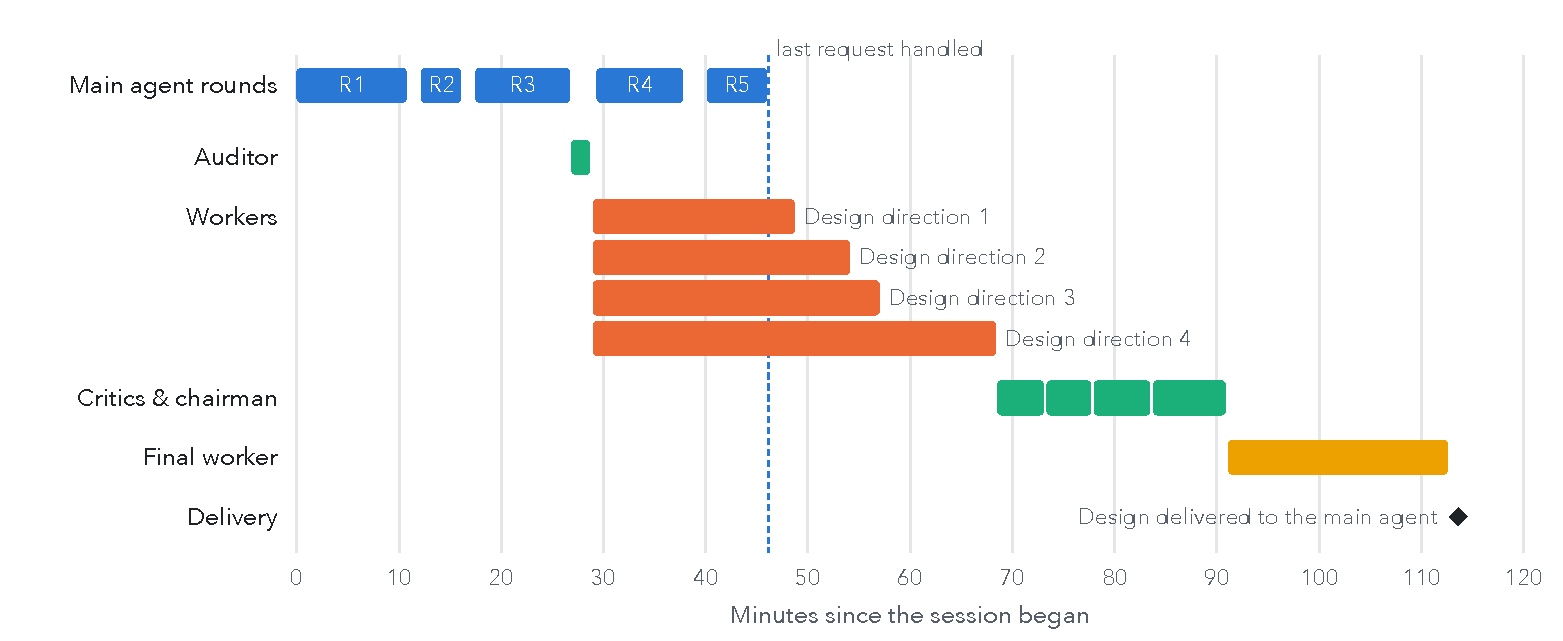
\includegraphics[width=0.88\linewidth]{fig_timeline.pdf}
  \caption{How a background run overlaps with a session. The user keeps working while the workers, the review and the final worker run, so a design can arrive well after the request that prompted it.}
  \label{fig:timeline}
\end{figure}

This doesn't happen on every request. That would create too much noise and disrupt the user's attention, and most requests are direct enough for the main agent to handle, or are simply questions for it. The intelligence of the system lies in figuring out when it makes sense to try something new, and in only sending something back when the redesign is useful.

The design also relies on cheap tokens. The background agents run open-source models in Sailboxes that bill only for what they use, so the user doesn't have to worry about a background system blowing up their costs. A system like this is enabled by cheap intelligence, and it becomes more useful as intelligence gets cheaper.

\section{Related Work}
\label{sec:related}

Exploring this problem turned up several research avenues aimed at the gaps and limitations of coding agents and their harnesses as they stand today. A few of them shaped this project directly.

The first is proactivity. Bui and Evangelopoulos at Google Labs argue that agentic coding needs proactivity as well as autonomy, with agents that ``may notice drift, uncertainty, or emerging opportunities before being asked''~\cite{bui2026proactivity}. They also treat human attention as a cost, saying an agent should avoid messages ``whose value is lower than their attention cost.'' Hindsight shares that view, and it is why so much of the design is about when to stay quiet.

The second is how agents respond to changes they didn't make. SWE-Touch benchmarks coding agents when users edit the code during a task~\cite{tan2026swetouch}. Conflicting edits lowered the average resolve rate on SWE-bench Verified by 7.7 percentage points, while helpful edits barely changed it, and 63.3\% of the audited failures ended with the conflict still in place. This matters here because a background design is also a change that arrives from outside the main agent's own work, so how the main agent reconciles it sits at the center of how the two systems interact.

The third is review. In Karpathy's llm-council, models give independent opinions, review each other anonymously, and a chairman decides~\cite{karpathy2025council}. It raises the questions any review step has to face: is the output of the review actually good, has it really been tested, and how can it be audited? The council was the inspiration for the review and return stage of Hindsight.

FeatureLoop offers a useful caution about the premise itself. Across 12 models, giving agents the full specification upfront led to 40.3\% success, against 51.6\% with progressive requests and 64.1\% with progressive requests plus correction~\cite{feng2026featureloop}. Giving an agent every requirement at the start may not be the full solution. That is one reason Hindsight doesn't replace the main agent, which keeps what it learned along the way and uses the redesign only as an addition to it.

Hindsight differs from this work in where it looks and who it answers to. It looks backward at a live session, and instead of working on the next request it asks what should have been built given everything so far. Nobody has to invoke it, and its output goes to another agent as a suggestion rather than to the user as a finished change.

\section{Methodology}
\label{sec:method}

The whole design comes down to one question: How should tasks be divided between the main agent and the background agents? Each is good at something the other can't do. The main agent knows the latest code, has learned the project's quirks and can talk to the user, but it built the code one request at a time and may be anchored on its early decisions. Background workers can try several structures in parallel, with nothing to protect, but they fall behind the conversation and can't ask the user questions. So the workers are given the full context up to that point, which lets them come in with a fresh perspective, and the judgment is left to the main agent and the user. That is why a design can be sent even when it is trailing behind the main conversation, since the main agent can reconcile it, and why a design only has to be worth reading, not ready to merge. The bar is still high: workers are prompted to come up with a better design, and several gates stop a bad or useless design from coming through. Ultimately, though, the main agent should think through what the background workers have given it and reach the final verdict with input and feedback from the user.

Figure~\ref{fig:flow} shows the four stages, and each section below explains what a stage does and how it got there.

\begin{figure}[t]
  \centering
  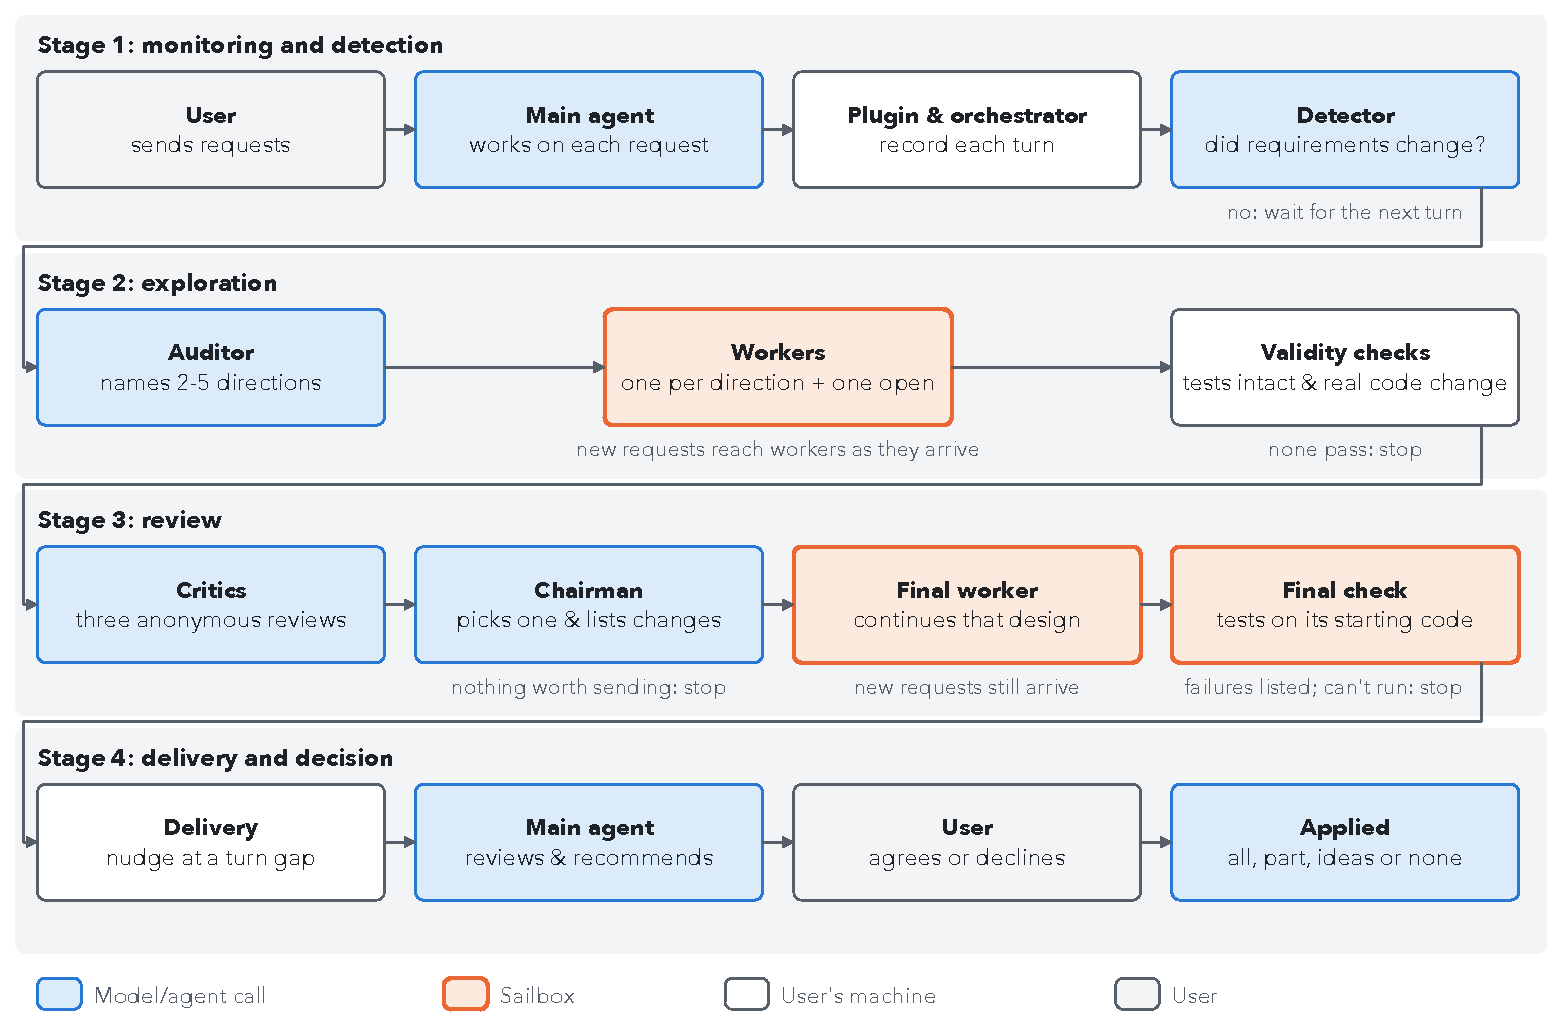
\includegraphics[width=0.8\linewidth]{fig_flow.pdf}
  \caption{The four stages of the system. Text under a box shows where a run can stop and where new requests reach a worker.}
  \label{fig:flow}
\end{figure}

\subsection{Stage 1: Monitoring and detection}

The user works with the main agent as usual. Hindsight uses OpenCode for this, watched through a plugin that forwards session events to the orchestrator, which runs on the user's machine. At the end of each turn, the orchestrator snapshots the folder to a private repository kept apart from the user's git history. The plugin never makes the session wait.

The harder problem is deciding when to act. One early design was an edge-case gate: models proposed edge cases the code might fail, ran them as real tests, and started the workers if any failed, which gave a trigger and a measurable target in one. The catch is that it's always possible to find an edge case. On a synthetic task designed to need no redesign, it delivered 17 nudges in 18 turns. It also pointed workers at problems a model had imagined instead of problems the user had, so it was dropped.

The opposite approach failed too. Another trigger asked the model whether it would build the code differently knowing everything, and it answered no on all 14 reviews across four benchmark tasks. Most of those requests added features without contradicting anything, and the code already worked. The current detector asks something narrower: does the latest request change or reverse something an earlier request specified, or something the code was built around (Figure~\ref{fig:request})? Purely additive requests count as no, and when unsure it answers yes. On a live run it said yes on 14 of 40 reviews, although a more robust evaluation would need a labeled set of ``redesign moments.''

\begin{figure}[t]
  \centering
  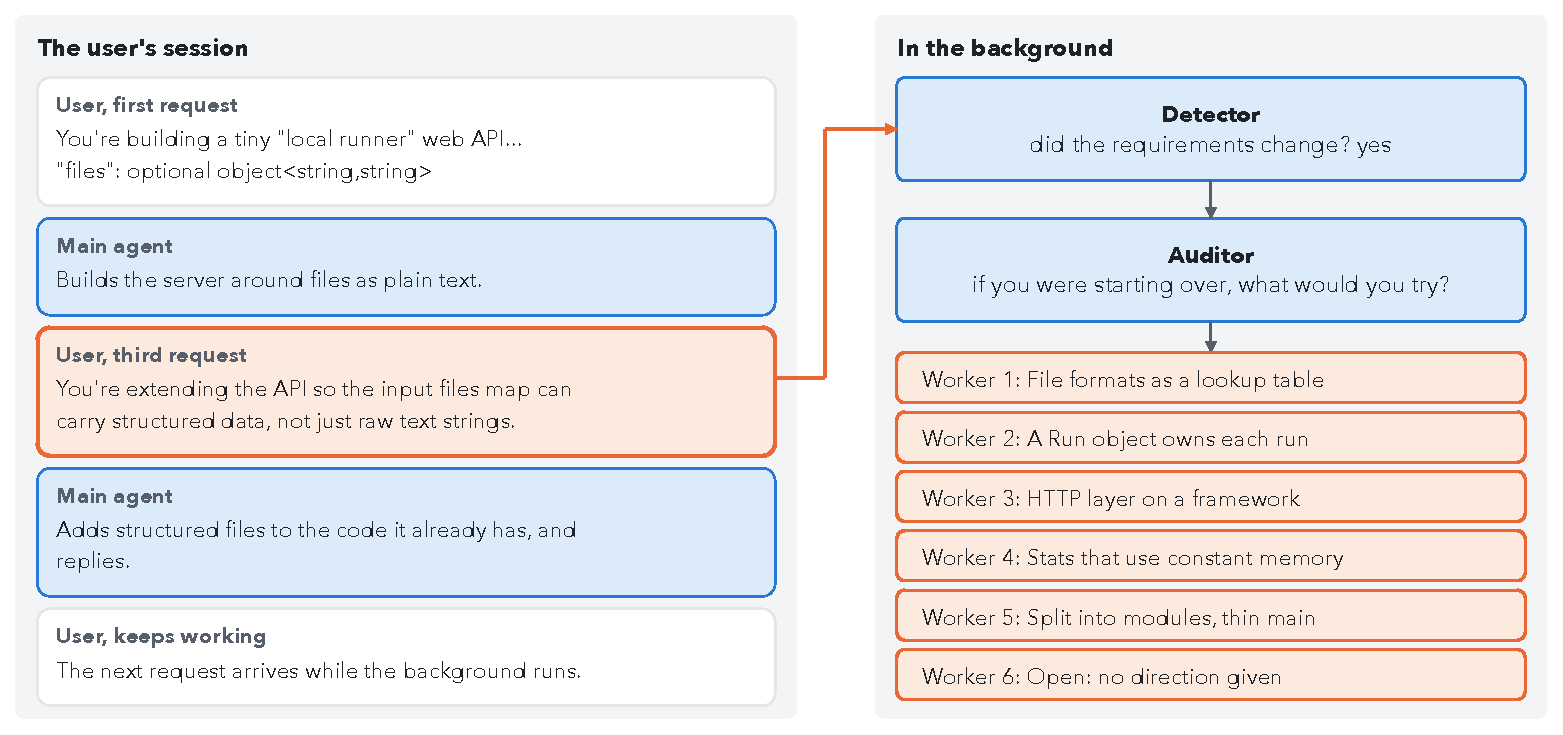
\includegraphics[width=0.9\linewidth]{fig_request.pdf}
  \caption{An illustrative example of a request that changes something the code was built around. The background starts while the session carries on. Messages are shortened from \code{execution_server}, a task from a public coding benchmark in which an agent builds a small web API for running code, and the directions are the ones the auditor named on that task.}
  \label{fig:request}
\end{figure}

\subsection{Stage 2: Exploration}

After a yes, an auditor names 2 to 5 directions a strong engineer would seriously consider if starting over. One worker builds each direction, and one more gets an open brief: nobody has picked a direction for it, so it is free to design whatever it would have built knowing everything. Each worker runs in its own Sailbox, a persistent Linux virtual machine billed for what it uses and free while asleep, with its own copy of the code. A worker can edit and run anything without going near the user's repository.

An earlier version used six fixed personas, such as a clean rewriter and a minimalist surgeon. They shared a step saying that leaving correct code alone was a useful result, and in one comparison 28 of 45 designs changed no real code. Now a worker has to restructure (``Handing back the same structure with a few fixes is not a result'') and has to say what its design makes better and what it costs. Letting the auditor set the number of workers means the team size follows the problem, though in practice it usually names close to the maximum.

Long-running workers raise the question of how to keep up with a conversation that doesn't stop. New user messages are delivered to every running worker, which reads them before finishing. Each session also runs only one background cycle at a time, since a second run would mostly repeat the first. The trade-off is that a weak run can stop a better one from starting.

Workers have a 45-minute time limit, which keeps runs feasible on complex tasks. This is a knob that can be tuned, and potentially set by the user, depending on cost and time constraints. A dropped connection continues the same conversation, and code present at the limit is kept and labeled unfinished. Two validity checks follow, using no model. One rejects weakened tests. The other requires a real change to product code, comparing Python by its syntax tree, because some designs only touched docstrings and config files.

\subsection{Stage 3: Review}

With several designs and no test that can say which structure is best, the review borrows the shape of Karpathy's llm-council~\cite{karpathy2025council}. Three critics, with the lenses requirements auditor, simplicity advocate and scope examiner, read the user's messages, the current code and each anonymized design. A chairman then picks one design to build on, or decides nothing is worth sending. It doesn't merge designs, because different structures rarely combine, but it lists what to change in the chosen design, which can include specific ideas borrowed from the others. A final worker starts with that design in place and makes those changes. Testing found that giving the final worker a design to build from, rather than asking it to redesign from a written plan, led to a better final design and better retained the workers' ideas.

The last step is a deliberately light check. Stricter checks would drop designs over changes that arrived late or over incompatibilities the main agent could resolve, and an early hard merge produced 48 false conflicts out of 48 proposals. So the check runs only against the code the design was built from, or runs the worker's own tests if the project has no suite, and a failure gets one retry. After that, the design goes out with its failures listed, because a test can fail only because it was tied to the old structure, and the main agent can tell the difference. Only a design that can't be run at all sends nothing.

\subsection{Stage 4: Delivery and decision}

At the next gap between turns, a nudge reaches the main agent, and the user gets a toast notification (Figure~\ref{fig:delivery}). The message is marked as coming from Hindsight and holds a one-sentence summary, an evidence line built by code, the background workers' own description labeled unverified, any messages the design missed, how far behind the design is, and the diff itself.

Delivery didn't start out this way. At first, a design needed a clean rebase and a test flip, then went straight to the user, all or nothing. Thinking through the relationship between the user, the main agent and the background system changed that. The main session doesn't wait, so suggestions will lag, which makes a strict, perfectly current patch the wrong thing to aim for, and the agent that has been in the code all along is the right reviewer.

The main agent reviews the design and recommends all of it, part of it, only its ideas, or none, and the user decides. The message asks the agent to change no code until the user agrees. Hindsight's own code only writes to the repository through an adoption tool, which takes a backup, runs tests and offers undo. Afterwards, the final worker's box goes to sleep, and the main agent can wake it to ask the background worker that built the design about it.

\begin{figure}[t]
  \centering
  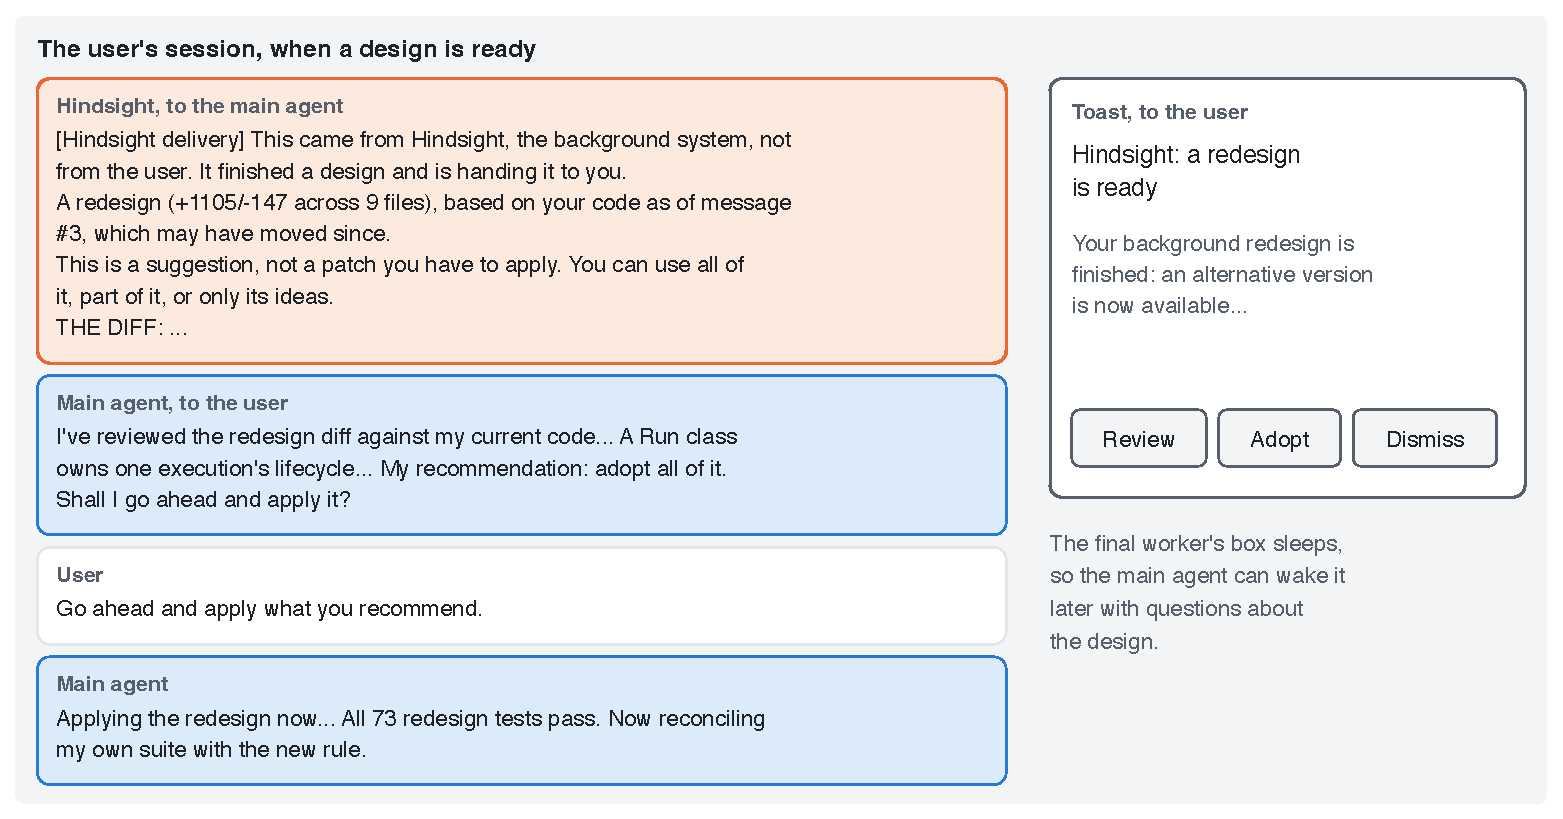
\includegraphics[width=0.9\linewidth]{fig_delivery.pdf}
  \caption{A design comes back. The main agent receives the diff and context, and the user gets a toast. Messages are shortened from \code{execution_server}, the web API task from Figure~\ref{fig:request}, where a simulated user gave the go-ahead. Benchmark runs have no desktop interface, so the toast is shown as designed.}
  \label{fig:delivery}
\end{figure}

\section{Evaluation and Early Results}
\label{sec:results}

A natural next step once the system was built was evaluating whether or not Hindsight was actually useful. This section walks through what was tried, why each approach gave way to the next, and a first comparison against an agent working alone.

\subsection{Starting with synthetic tasks}

The first tasks were synthetic projects given to the agents with simple evolving requirements, like an expense log that had to adjust to show the purchases behind its totals. This proved not to be a great evaluation, as the requirement changes were too small to need a real redesign, and bugs in the tasks and the system’s own pipeline muddied the results.

\subsection{Moving to public benchmarks}

SlopCodeBench~\cite{orlanski2026slopcode} became the main benchmark because of how closely it matches the problem. An agent extends its own code through a sequence of specifications, and it is graded with hidden tests plus two quality scores, verbosity and structural erosion. Fitting a background system into it still forced a choice about what was really being measured:

\begin{itemize}[nosep]
  \item \textbf{Time.} This was the biggest issue. Benchmarks assume the next request can arrive whenever the agent finishes. A median round took 10 to 26 minutes, while a background run took about 1.5 to 2 hours, so a benchmark that doesn't wait mostly measures lateness. The runner can hold the next request until a design arrives, which tests whether a design helps when it lands in time, and every hold is recorded because a real user wouldn't wait.
  \item \textbf{What the scores reward.} Adding tests alone moved verbosity from .28 to .14 on unchanged code, so quality is re-scored without test files. Hidden tests reward behavior, while Hindsight aims at structure, so a good redesign may not move them at all.
  \item \textbf{The user and the conversation.} A custom runner keeps the conversation across rounds, as in a real session, so scores can't be compared with published leaderboards. A simulated user answers the agent's recommendations and always agrees, which says nothing about real users.
  \item \textbf{Noise.} Identical agents on the same task can differ a lot: the median difference between copies was .156 in erosion. One run per task can only detect a large effect.
\end{itemize}

\subsection{Comparing four setups}

The last run was a small experiment to test the value of Hindsight. Ten SlopCodeBench tasks were drawn at random and run in four setups, with the plan written down beforehand: the agent alone (A), Hindsight forced at each task's middle round (B), and Hindsight whenever the detector says yes, with the next request either arriving on schedule (C) or held until the background run ends (D).

No setup clearly beat the agent working alone (Table~\ref{tab:compare}). Each won about half the tasks on most scores, and D's lead on verbosity, 7 of 9, was the same after the first round, before any design existed. Designs still reached the agent 23 times, and in some cases they helped: several found real bugs that the agent confirmed and fixed, and it took a whole design about 6 times and part of one about 11 times. It also judged them critically. On \code{metric_transform_lang} in C, where requests didn't wait, it turned a design down because it was ``two messages stale'' and ``would have destroyed the finished Part 4/5 work.'' On \code{pwd_manager} in D, it recommended ``Adopt all of it'' and then applied the design without waiting for the user, a reminder that the instruction to wait isn't enough on its own.

The experiment has clear limits. Each task ran once per setup, and single runs differ about as much as the setups did, so a much bigger sample is needed before anything can be said about quality. The simulated user always agreed, every role used the same model, the tasks had been seen in earlier runs, and holding requests until a design arrives is not what a real user would do. The scores also reward behavior more than structure, which is what Hindsight is trying to improve.

\begin{table}[t]
  \centering
  \small
  \begin{tabular}{@{}l c c c c@{}}
    \toprule
    & \textbf{Designs} & & & \textbf{Hidden} \\
    \textbf{Setup} & \textbf{delivered} & \textbf{Erosion} & \textbf{Verbosity} & \textbf{tests} \\
    \midrule
    B. Forced, waits & 7 & 5 of 9 & 5 of 9 & 4 of 9 \\
    C. Detector, on schedule & 6 & 5 of 9 & 7 of 9 & 2 of 9 \\
    D. Detector, waits & 10 & 4 of 9 & 7 of 9 & 4 of 9 \\
    \bottomrule
  \end{tabular}
  \caption{Tasks where each setup did better than the agent working alone, out of the nine scored in every setup. Erosion measures how much complexity piles up in a few places, verbosity measures repeated and padded code, and both are scored without test files at the end of the session, where lower is better. Hidden tests are the benchmark's tests, where more passing is better.}
  \label{tab:compare}
\end{table}

\section{Next Steps}
\label{sec:discussion}

As I continue working on this, my first priority is to find better ways to measure the system. The question I care about is whether code that takes a redesign is easier to extend later on, and today's benchmarks only get at that indirectly. I want to design an evaluation around that question and put the system in front of real people to see how it performs in the wild. A poor evaluation can make a great product look bad or pull it toward the wrong goal, and real usage would give me the feedback I need to keep breaking things and making the system better.

I also want Hindsight to adapt to each person who uses it. It should learn their preferences from the designs they accept and turn down, and it should learn when they are away from the keyboard so it can start more background runs during those hours. It should also draw on more than the coding session, using sources like Slack messages and meeting notes to suggest changes based on a fuller picture of the work. The north star is a background agent that keeps learning from the person it works with: one that gets more useful with every decision they make, notices what matters before being asked, and makes progress for them while they are away.

\section{Conclusion and Final Reflection}
\label{sec:conclusion}

\paragraph{Making use of the tools available.}
This project was really my first time working with open-source models and an open-source harness. They weren't as intelligent as the frontier models I was used to, but they were a lot cheaper, so I could delegate longer tasks to them and run things overnight. Working with Sailboxes taught me something similar. They made it cheap to run many isolated workers, but I had to learn how they fail, from boxes left running when a process was killed partway through creating them, to limits on reserved CPU that stopped workers while actual usage was close to nothing. Any project is going to have constraints, and a big part of my learning is to continue to discover how to best use the tools available for any given task.

\paragraph{Simplicity versus complexity.}
As I designed the system, I thought very deeply about the best user experience, and there were a million edge cases to consider. When does it make sense to alert the user? Should I alert the user or the agent? Should there be a minimum number of turns before sharing a design? Should multiple background processes run at the same time? Should the orchestrator run in a Sailbox or on my computer? The list goes on. The more edge cases I fit to, the more complex the system became and the better it could adapt to what real users might do, but the law of unintended consequences holds strong: you fix one thing and you might end up breaking thirty others. I don't think there is a perfect middle point between the two extremes, and it's something any great product has to confront.

\paragraph{Letting the data decide.}
This is a lesson I learned from my first manager at Databricks, and it comes back to me in almost every project I do. Perfect decisions and designs don't exist, and whether a design sticks is tied to user bias and all sorts of other things, so one of the most defensible things you can do when designing any system is let the data decide. In this project, that meant testing different prompt variations on real coding problems and tracking the spend and time of evaluation runs, and it's something I will continue to think about as I build more products in the future.


{\small
\bibliographystyle{plainnat}
\bibliography{references}
}


\end{document}
